\documentclass[a4paper,11pt]{article}
\usepackage[utf8]{inputenc}
\usepackage[T1]{fontenc}
% Mes polices: times, newcent, default
\usepackage{times} % problème d'accent avec charter
\usepackage[top=2cm, bottom=2cm, left=2cm, right=2cm]{geometry}
\usepackage{array}
\usepackage{graphicx}
\title{Rapport intermédiaire}
\author{Yasin Arslan}
\date{15 décembre 2014}

\setlength{\parindent}{0cm}
\setlength{\parskip}{1ex plus 0.5ex minus 0.2ex}
\newcommand{\hsp}{\hspace{20pt}}
\newcommand{\HRule}{\rule{\linewidth}{0.5mm}}

\begin{document}

\begin{titlepage}
  \begin{sffamily}
  \begin{center}

    \textsc{\LARGE \textit{Université Libre de Bruxelles}}\\[0.3cm]
    \textsc{\LARGE \textit{Rapport intermédiaire}}\\[2cm]
    \textsc{\LARGE \textbf{INFO F-106}}\\[0.3cm]
    \textsc{\LARGE \textbf{Projet d'informatique}}\\[2cm]


    \HRule \\[0.4cm]
    { \huge \bfseries Propagation de la rumeur\\[0.4cm] }

    \HRule \\[2cm]

    \begin{minipage}{0.4\textwidth}
      \begin{flushleft} \large
        ARSLAN \textsc{Yasin}\\
        MATRICULE : \textsc{000396506}\\
      \end{flushleft}
    \end{minipage}
    \begin{minipage}{0.4\textwidth}
      \begin{flushright} \large
        \emph{Tuteur :} M. \textsc{Gwenaël Joret}\\
        \textsc{2014-2015}\\
      \end{flushright}
    \end{minipage}
    \\[2cm]
    
\includegraphics{image.jpg}
    \vfill
    {\large Fin de la rédaction le 4 avril 2015}

  \end{center}
  \end{sffamily}
\end{titlepage}

\renewcommand{\contentsname}{Table des matières}
\tableofcontents
\newpage

\section {Introduction}

\paragraph{}
{Dans le cadre du cours \textbf{projet\ d'informatique},il nous a été demandé d'implémenter en \textbf{python3} un simulateur de propagation d'une rumeur dans un réseau d'amis.
Ce projet est divisé en 4 grandes parties. Ce rapport va résumer les deux premières. La partie 1 consistait principalement à la création du réseau et la propagation d'une rumeur dans ce réseau.
La partie 2 va apporter une toute autre diversité en offrant à l'utilisateur une liberté lors de l'exécution. La 3ème partie permet l'éxécution via une interface graphique ainsi que sur terminal,
tandis que la 4ème partie va renforcé l'interface graphique sans pour autant ajouter des fonnctionnalités à la partie terminal.
Mis à part l'introduction et la conclusion,le corps du rapport sera divisé en 3, une pour chaque partie et la troisième détaillera mes propositions pour la partie 4.
Une analyse des fonctions et structures utilisés ainsi que quelques commentaires y seront disponibles.
J'ai décidé d'écrire mon code en anglais. Le langage n'était pas imposé mais l'anglais étant la langue internationale, j'ai trouvé son utilisation plus approprié.}
\paragraph{}
{Pour la $1^{\textrm{ère}}$ partie, La simulation débutait en demandant à l'utilisateur le nombre d'étapes de simulation, le nombre de personnes dans le réseau et leurs noms.
Grace à cette dernière information, le simulateur va pouvoir demander le lien d'amitié entre ces personnes. Il faudra entrer 1 s'ils sont amis, 0 sinon. Plus le réseau était peuplé, plus cette étape prenait du temps. Finalement,
il sera demandé la personne à l'origine de la rumeur. Cette personne devra être dans le réseau sinon on redemande à nouveau. La création du réseau étant terminé et la rumeur ayant été initié, la simulation pouvait avoir lieu.}
\paragraph{}
{Pour la $2^{\textrm{ème}}$ partie, les inputs vont disparaitre et laisser place aux arguments. La tache de l'utilisateur est donc allégée.
Le réseau va se charger via un fichier texte dans le même répertoire que notre programme. Celui-ci sera donné en argument. 
On suppose le fichier étant correcte, 
c'est à dire que les lignes sont écris comme suit et qu'il n'existe aucune incohérence :
\newline -----------------------
\newline Alice : Bob,David
\newline Bob : Alice
\newline David : Alice
\newline -----------------------
\newline Nous avons également attribué à la rumeur une valeur qui sera un nombre sur 8 bits (0 à 255). De cette manière, on a ajouté des fonctionnalités
 qui permettent de modifier la rumeur. La partie 2 du rapport expliquera en détails comment utiliser ces fonctionnalités.}
\paragraph{}
{La $3^{\textrm{ème}}$ partie a introduit un tout nouveau mode d'éxécution. Celui-ci propose à l'utilisateur une interface GUI avec lequel il peut interagir.
L'introduction de ce nouveau mode d'éxécution n'éxclue pas le premier, qui corresponds à l'éxécution sur terminal. 
Dans cette interface, On y trouve divers bouttons et listes pour choisir les options de propagation et créer le réseau.
Ce mode a également introduit les classes python. Il nous a été demandé de créer 4 nouvelles classes :
\newline - GUI : Cette classe encapsule l'interface graphique et toutes les fonctionnalités liées qui seront expliqués dans la section correspondante.
\newline - NetworkFrame : Dans le GUI se trouve une partie dessin que l'on appelle canvas. C'est là que nous pourrons voir le réseau ainsi que les rumeurs.
\newline - Person : Cette classe crée une personne sur le réseau et dessine un oval sur le canvas.
\newline - Link : Via le système Drag-and-Drop , il est possible de créer un lien d'amitié entre deux personnes. Cette classe va s'occuper de dessiner ces liens sur le canvas.
\newline La rumeur qui était sur 8 bits passe à 24. Celle-ci sera représenté par une couleur tel que les  3 bytes représentent respectivement les valeurs RGB. 
Pour l'éxécution standart sur terminal, il n'y a que la taille de la rumeur qui change. Celle-ci est éxécutable via le fichier rumor.py.}
\paragraph{}
{La $4^{\textrm{ème}}$ partie donnait la liberté de choisir entre diverses fonctionnalités outre deux imposés. La sauvegarde et restauration du réseau était la première 
et les statistiques globales la seconde. Parmis la liste des choix, j'ai choisi la fonctionnalité "Envoyer à tout les amis","Création de réseau via l'interface" et "Cluedo".}
\newpage
\section{Création des structures de données et fonctions de base }

\subsection{Présentation}
\paragraph{}
{Pour commencer, tout le réseau est créé manuellement via des inputs.
3 structures et 4 fonctions principales ont été imposées et seront détaillés dans la section correspondante.
J'ai également choisi de diviser mon code en plusieurs sous-fonctions.
L'exécution du programme s'effectue via une fonction main.}
\subsection{Structures}
\paragraph{names\newline}
{La liste des noms de chaque personne dans le réseau dans l'ordre des inputs donnés.}
\paragraph{InformedPeople\newline}
{Une liste de booléen qui représente la connaissance de la rumeur pour chaque personne.
Tel que InformedPeople[i] représente la connaissance de names[i]. True si elle connait la rumeur, False sinon.}
\paragraph{network\newline}
{La matrice représentant la relation de chaque personne dans le réseau entre elles.
Tel que network[i][j] représente la relation entre names[i] et names[j]. True s'ils sont amis, False sinon.
Nous avons supposé une symétrie tel que si A est ami avec B, B est ami avec A.}

\subsection{Fonctions}
\subsubsection{Fonctions principales}
\paragraph{inputData\newline}
{Initialise names et network via les fonctions input\_names et users\_frienship. Cette fonction ne prend aucun paramètre.
Retourne names et network.}

\paragraph{PrintStates\newline}
{Affiche l'état du réseau. Cette fonction prends names et InformedPeople en paramètre.\newline
Affiche l'état du réseau en utilisant une boucle for avec indice pour chaque personne dans le réseau. Si InformedPeople a cet indice est True, 
on affichera que cette personne connait la rumeur, sinon on affiche qu'elle ne connait pas la rumeur.}

\paragraph{update\newline}
{Propage la rumeur et mets à jour InformedPeople. Cette fonction prend network et InformedPeople en paramètre.
On va créer une nouvelle liste NewInformed qui sera une copie d'InformedPeople comme ça nous pourrons modifier l'une sans pour autant modifier l'autre.
Si on modifiait InformedPeople, une personne ne connaissant pas la rumeur au début de l'étape pourrait la transmettre à un ami lors de la même étape.
Mise à jour des personnes informés tel que chaque étape, les personnes connaissant la rumeur la transmette à un ami.
Cet ami pourrait déjà connaitre la rumeur et la réentendre.
Retourne rumor\_spread qui représente le nombre de personne ayant appris la rumeur. Le calcul est effectué par un count entre les deux listes.
L'une étant initiale l'autre ayant été modifié. Cette fonction a été modifiée par la suite dans la partie 2.}

\paragraph{main (Exécution )\newline}
{Regroupe les fonctions et s'exécute. Ne prends aucun paramètre.
Fait appel à la fonction create\_rumor. Une fois cette rumeur créée, on affiche l'état initial.
Demande un input du nombre d'étape qui doit être un entier positif que l'on assignera à la variable simule.
Ensuite on initialise names et network avec la fonction InputData que nous avons défini plus tôt.
Pour éviter du travail inutile, si le réseau est vide, le programme se termine. Sinon, On va initier InformedPeople.
Initialement personne ne connait la rumeur donc on utilise un booléen False.
Ensuite on crée la rumeur et on enclenche la boucle principale de simulation qui va mettre à jour et ensuite afficher le réseau simule fois.}
\subsubsection{Fonctions supplémentaires}
\paragraph{input\_names\newline}
{Demande à l'utilisateur le nom de chaque personne et l'ajoute dans une liste. Cette fonction prend users en paramètre.
Cette variable représente le nombre de personnes dans le réseau.\newline
Retourne names qui est la liste des noms de chaque personne.}
\paragraph{user\_friendship\newline}
{Demande à l'utilisateur toutes les relations dans le réseau. Cette fonction prend names en paramètre.
Grâce à la symétrie des relations, le travail de cette fonction est allégé.
Retourne la matrice network.}
\paragraph{create\_rumor\newline}
{Demande à l'utilisateur une personne du réseau qui sera à l'origine de la rumeur.
Cherche l'indice de cette personne dans names tel que names[indice] représente le créateur.
Modifie cet indice dans InformedPeople et affiche l'état du réseau avec PrintStates.}
\subsection{Exemple d'exécution}
\paragraph
{--------------------------------------------------------------------------------
\newline Number of steps of the simulation : \textbf{1}
\newline Enter the number of people in the network : \textbf{3}
\newline Enter the name of the 1 person : \textbf{Alice}
\newline Entre the name of the 2 person : \textbf{Bob}
\newline Enter the name of the 3 person : \textbf{Yasin}
\newline Alice and Bob are friends (1 if yes, else 0) : \textbf{1}
\newline Alice and Yasin are friends (1 if yes, else 0) : \textbf{0}
\newline Bob and Yasin are friends (1 if yes, else 0) : \textbf{1}
\newline Enter the person at the origin of the rumor : \textbf{Yasin}
\newline \#\#\#
\newline Initial:
\newline Alice doesn't know the rumor.
\newline Bob doesn't know the rumor.
\newline Yasin knows the rumor.
\newline \#\#\#
\newline Step 1:
\newline Alice doesn't know the rumor.
\newline Bob knows the rumor.
\newline Yasin knows the rumor.
\newline --------------------------------------------------------------------------------}

\section{Fonctionnalités supplémentaires sur terminal}
\subsection{Présentation}
\paragraph{}
{Une liberté est née dans le simulateur grace à ces fonctionnalités.
Le but principal étant de modifier la rumeur et d'y mettre des conditions de propagation.
La rumeur devient une valeur sur 8 bits. Nous allons modifier et utiliser 2 fonctions qui sont update et PrintStates,
et les structures seront conservé mais modifié quelque peu. Pour présenter cette partie, il faut introduire les librairies
 utilisées ainsi que les fonctionnalités proposés. Les fonctions principales et les changements seront également expliqués.}
\subsubsection{Librairies}
\paragraph{Argparse\newline}
{La libraire argparse permet de prendre des arguments donné dans un ordre quelconque et de les regroupé comme voulu.
Ici la tache de argparse sera principalement de stocker les valeurs pour une utilisation dans le code. Si aucune valeur n'est 
donné, par défaut elle vaudra None. Grâce à ça, nous pourrons utilisés les fonctionnalités donné par l'utilisateur ou 
exécution le code par défaut.}
\paragraph{Random\newline}
{Nous utiliserons random et randint de cette libraire. Le premier génère un nombre entre 0.0 et 1.0, le deuxième demande 
deux paramètres qui seront les bornes comprises de la génération demandée.}
\subsubsection{Fonctionnalités}
{Pour l'utilisation des fonctionnalités il faudra les introduire en arguments sinon le programme s'exécutera par défaut.
Néanmoins, un argument reste obligatoire, c'est le document contenant le réseau. Via celui-ci le réseau sera chargé.
8 possibilités d'arguments sont donnés, les voici :\newline
--------------------------------------------------------------------------------------------------------------------
\newline\textbf{-h :} Affiche une aide d'exécution. \textbf{Defaut :} N'affiche pas l'aide.
\newline\textbf{-s Person :} "Person" devient le créateur de la rumeur. \textbf{Défaut :} Une personne aléatoire.
\newline\textbf{-r Rumor :} Le créateur de la rumeur crée "Rumor". \textbf{Défaut :} Un nombre aléatoire de 0 à 255.
\newline\textbf{-t Simule :} Propage la rumeur "Simule" tours. \textbf{Défaut :} S'arrête quand tout le monde connait la rumeur.
\newline\textbf{-d :} Une personne connaissant déjà la rumeur ne peut la réentendre. \textbf{Défaut :} Il peut la réentendre.
\newline\textbf{-m Rule :} La rumeur sera modifié de la manière "Rule". \textbf{Défaut :} La rumeur ne se modifie jamais.
\textbf{Posibilités :} "none" : Pas de modification ; "incremental" : La rumeur est augmenté ou diminué de 1 ;
"bitflip" : un bit aléatoire de la rumeur est changé sur 2 bits.
\newline\textbf{-p X :} Probabilité "X" que la rumeur soit modifié lors de la transmission. \textbf{Défaut :} X = 0.1
\newline\textbf{-u Rule :} La transmission de la rumeur se fait de la manière "Rule". \textbf{Défaut :} stable.
\newline\textbf{Possibilités :} "stable" : Une personne connaissant la rumeur ne verra jamais sa connaissance modifiée.
"rewrite" : Chaque fois qu'une personne apprends la rumeur, il la fait sienne. \newline"mixture" : Création d'une nouvelle rumeur à partir 
de la comparaison bit à bit du réceptionneur et du transmetteur. Si le bit est identique on l'ajoute, sinon on procède à un random 
avec 9 chances sur 10 de conservé le bit du réceptionneur et 1 chance sur 10 de la modifier.
\newline--------------------------------------------------------------------------------------------------------------------}

\subsection{Nouveautés}
\subsubsection{Binaire}
\paragraph{}
{Pour l'écriture en binaire, j'ai utilisé un format de chaîne de caractères. Ce format transforme un nombre entier en binaire 
sur 8 bits et le renvoie en chaîne de caractère. Cette méthode a facilité l'utilisation de la modification bitflip ou encore 
la méthode de transmission mixture.}
\subsubsection{Chargement du réseau}
\paragraph{}
{Une fonction \textbf{LoadNetwork} a été codé pour prendre en paramètre le fichier texte donné en argument et 
s'occupe d'initier la liste des noms et la matrice du réseau. On prends soin de nettoyer les espaces inutiles pour chaque 
ligne.}
\subsection{Modification de la partie 1}
\subsubsection{Structures}
\paragraph{}
{Pour les structures, j'ai décidé de modifier network tel qu'une personne n'est plus ami avec elle-même.
De la sorte, j'évite une vérification inutile et une personne connaissant la rumeur ne puisse la transmettre à elle-même.
\newline Ensuite InformedPeople va être initié plus à False mais à None. Un None étant plus propre et léger.
Et les indices des personnes connaissant la rumeur ne seront plus à True, mais auront la valeur entière de cette rumeur.}
\subsubsection{Fonctions}
\paragraph{Printstates\newline}
{Printstates va maintenant afficher le nom de la personne suivie de sa connaissance binaire et entière de la rumeur.
S'il ne connait pas la rumeur une information l'indiquera.}
\paragraph{update\newline}
{Le déroulement va complétement être mis à jour. Avec la modification introduite dans cette partie, Nous allons y ajouter 
les 3 valeurs de nos arguments "-d" ,"-m" et "-u" . La première nous informera si oui ou non on peut transmettre la rumeur à
une personne la connaissant déjà via un booléen. La seconde va modifier ou non la rumeur par la méthode demandée et la troisième 
va la transmettre avec les instructions données.}
\subsubsection{Paramètres}
{Avec l'introduction des arguments, nous avons du ajouter à nos fonctions les arguments nécessaires à l'utilisation.
Certains fonctions prenant trop d'argument, il a été préféré de mettre la variable regroupant tout les arguments et utiliser
celle voulue ensuite. De la sorte le code est plus lisible et garde la même compréhensibilité mais en revanche on perd un peu
d'efficacité.}
\subsection{Nouvelles fonctions}
{Plusieurs nouvelles fonctions ont vu jour. Mis à part les fonctions les regroupant, voici la liste :
\newline \textbf{takeArgs()} : Prends les arguments donnés et les mets en groupe via Argparse.
\newline \textbf{verifyArgs(args)} : Vérifie Rumeur [0,255],Proba[0.0,1.0],Simule[0,+].
\newline \textbf{incremental(rumor\_number)} : Incrémente ou décrémente la rumeur de 1 avec une probabilité égale.
\newline \textbf{bitflip(rumor\_number)} : Inverse l'un des 8-bits de la rumeur.
\newline \textbf{everyone\_know(names,network,InformedPeople,args)} : Simule jusqu'à ce que tout le monde connait une rumeur.
\newline \textbf{number\_simulate(names,network,InformedPeople,args)} : Simule la propagation le nombre de fois donné en argument.
\newline \textbf{updateRules(NewInformed,rumor,chosenOne,updateRule)} : Transmet la rumeur via les instructions demandés.}
\subsection{Exemple d'exécution}
{\textbf{
python3 rumor.py -m incremental friend.txt -u rewrite -p 0.9 -s Alice -r 255
\newline -------------------------------------------------------------------------------------------------
\newline - - - - - - - -The Network- - - - - - - -
\newline Alice : Bob,David,Eve
\newline Bob : Alice,David
\newline David : Bob,Alice
\newline Eve : Alice
\newline
\newline Rumor starter : Alice
\newline Initial rumor : Alice
\newline \#\#\#
\newline Initial :
\newline \#Name\# \hspace{1.3cm} \#Bin\# \hspace{1cm} \#Num\#
\newline Alice \hspace{1.5cm} 11111111 \hspace{1cm} 255
\newline Bob \hspace{1.7cm} - - doesn't know - -
\newline David \hspace{1.4cm} - - doesn't know - -
\newline Eve \hspace{1.7cm} - - doesn't know - -
\newline \#\#\# Simulation step : 1
\newline - - > 1 learned the rumor this step
\newline \#Name\# \hspace{1.3cm} \#Bin\# \hspace{1cm} \#Num\#
\newline Alice \hspace{1.5cm} 11111111 \hspace{1cm} 255
\newline Bob \hspace{1.7cm} - - doesn't know - -
\newline David \hspace{1.4cm} - - doesn't know - -
\newline Eve \hspace{1.7cm} 00000000 \hspace{1.2cm} 0
\newline \#\#\# Simulation step : 2
\newline - - > 1 learned the rumor this step
\newline \#Name\# \hspace{1.3cm} \#Bin\# \hspace{1cm} \#Num\#
\newline Alice \hspace{1.5cm} 11111111 \hspace{1.1cm} 255
\newline Bob \hspace{1.7cm} - - doesn't know - -
\newline David \hspace{1.3cm} 11111110 \hspace{1.1cm} 254
\newline Eve \hspace{1.7cm} 00000000 \hspace{1.2cm} 0
\newline \#\#\# Simulation step : 3
\newline - - > 1 learned the rumor this step
\newline Alice \hspace{1.45cm} 00000001 \hspace{1.2cm} 1
\newline Bob \hspace{1.6cm} 00000000 \hspace{1.2cm} 0
\newline David \hspace{1.3cm} 11111110 \hspace{1.1cm} 254
\newline Eve \hspace{1.7cm} 00000000 \hspace{1.2cm} 0
\newline -------------------------------------------------------------------------------------------------
}
\newpage
\section {Interface graphique}
\subsection {Présentation}
{Comme dit dans l'introduction, une éxécution via interface graphique est possible. Dans celui-ci, les options de propagation 
et modification sont conservées et peuvent être changées en cours d'éxécution. Voilà une des grandes différence avec le terminal ou il suffisait 
de taper une ligne de commande. Ici il est possible d'interagir avec l'interface a tout moment.}
\subsection {Représentation sur le canvas}
\subsubsection {Utilisateur}
{Un utilisateur est représenté par un oval sur le canvas. Sa taille est modifiable via la valeur de "Modify weight".}
\subsubsection {Lien d'amitié}
{Lorsque l'on veut voir les relations d'une personne, il faut la survoler. Chaque personne possède une ligne rouge pour montrer que 
les liens representent la liste d'amitié de cette personne. Ses liens d'amitié sont représentés en bleus et je rejoigne tous au centre.}
\subsubsection {Rumeur}
{La rumeur est donc un nombre représenté sur 24 bits. Chaque byte représente une couleur RGB. Et donc la rumeur de chaque personne est 
représenté par la couleur de son oval.}
\subsection {Création manuel du réseau via interface}
\subsubsection {Création des utilisateurs}
{Un utilisateur du réseau est représenter par un oval sur l'interface. Pour le créer, il suffira d'appuyer sur le boutton "Add node" 
pour ouvrir une boite de dialogue demandant le nom de la personne. Attention on ne peut pas utiliser le même nom plus d'une fois, pour aider l'utilisateur,
une liste avec les noms déjà utilisés est disponible dans cette boite de dialogue.
Un rond sera tracé sur le canvas en pointillé pour montrer à l'utilisateur à quel place se trouvera cette nouvelle personne.}
\subsubsection {Création des relations d'amitiés}
{Pour ajouter une personne B dans la liste d'amitié de la personne A, il suffit de faire survoler l'ovale représentant la personne A et la déposer 
sur l'oval de la personne B. Ainsi A est ami avec B sans pour autant que B n'est ami avec A. C'est via ces relations que la rumeur 
va se propager dans le réseau.}
\subsection {Création manuel du réseau via boite de dialogue}
{Dans la barre de menu "custom", il est possible de créer le réseau via une succession de boite de dialogue.
Tout d'abbord, le nombre de personne sera demandé et une succesion de boite de dialogue demandant le nom pour chaque personne 
ensuite pour chaque personne, ses relations d'amis.}
\subsection {Création automatique du réseau}
{Dans le barre de menu "custom", en entrant le nombre de personne, il est possible de créer un réseau avec des utilisateurs et des liens d'amitié 
totalement aléatoire. Les noms seront aléatoire avec une taille minimum de 1 caractère et une taille maximum de 8. Pour les liens d'amitié, 
chaque personne a 1 chance sur 2 d'être ami avec une autre personne.}
\subsection {Chargement du réseau via un fichier}
{Il est possible via la barre de menu, de charger un réseau déjà enregistré dans un fichier texte. Celui-ci doit respecté la syntaxe imposé.
La première ligne représente les derniers paramètres de propagation enregistré dans le réseau chargés.
Les lignes qui suivent ont une syntaxe basique représentant chaque utilisateurs et pour chaque utilisateur, ses amis.}

\subsection {Exclusivité interface graphique}
\subsubsection {Sauvegarde du réseau}
{Il est possible de sauvegarder l'entièreté du réseau ainsi que les options de propagation via la barre de menu. La sauvegarde s'effectue sur un fichier txt.
Il est également possible par la suite de charger ce réseau dans le même menu.}
\subsubsection {Statistiques}
{Il est possible d'afficher des statistiques via le boutton "Statistics" ou lors de la création d'un réseau via la barre de menu "custom".
Dans celle-ci se trouve l'étape courrante, le nombre de personnes dans le réseau, le nombre de personne connaissant la rumeur/ne connaissant pas la rumeur,
le nombre minimum/maximum d'amis d'une personne et le nombre d'amis en moyenne dans le réseau. Il y a également des statistiques individuelles soit 
les amis ainsi que les anciens amis soit la rumeur actuelle et les anciens rumeur pour chaque personne.}
\subsubsection {Envoyer à tous}
{Une option de propagation exclusive à l'interface graphique, lors de chaque étape de simulation, une personne va dire la rumeur non plus 
à un ami aléatoire, mais à tout ses amis. La rumeur que la personne apprendra sera celle qu'il aura le plus entendu cette étape sinon une au hasard 
parmis celle entendu. Pour activer cette option, il suffit de cocher la case "send to all friends".}
\subsubsection {Cluedo}
{La rumeur n'est plus un nombre, mais la réponse à la question : “Qui a tué le Docteur Lenoir, dans quelle pièce du manoir et avec quelle arme a été commis le
meurtre ?”. L'utilisateur peut activer le cluedo et modifier les possibilités de réponse via la barre de menu "cluedo".}
\subsubsection {Modification du réseau}
{A tout moment, il est possible à tout moment lors de la simulation de supprimer une personne mais d'autre modifications sont également disponible.
Mais pour se faire, il faut que la propagation n'est pas commencée, c'est à dire l'étape de simulation doit être à 0. Si la rumeur a déjà été lancé, 
il faudra appuyer sur le boutton "reset steps" qui garde l'état courant du réseau mais réinitialise l'étape à 0. A partir de là,
il est possible d'ajouter de nouvelle personne, de modifier les rumeurs ou encore modifier les liens d'amitiés de chaque personne.}

\subsection{Annexe}
\subsubsection{Exemple de réseau avec lien d'amitié}
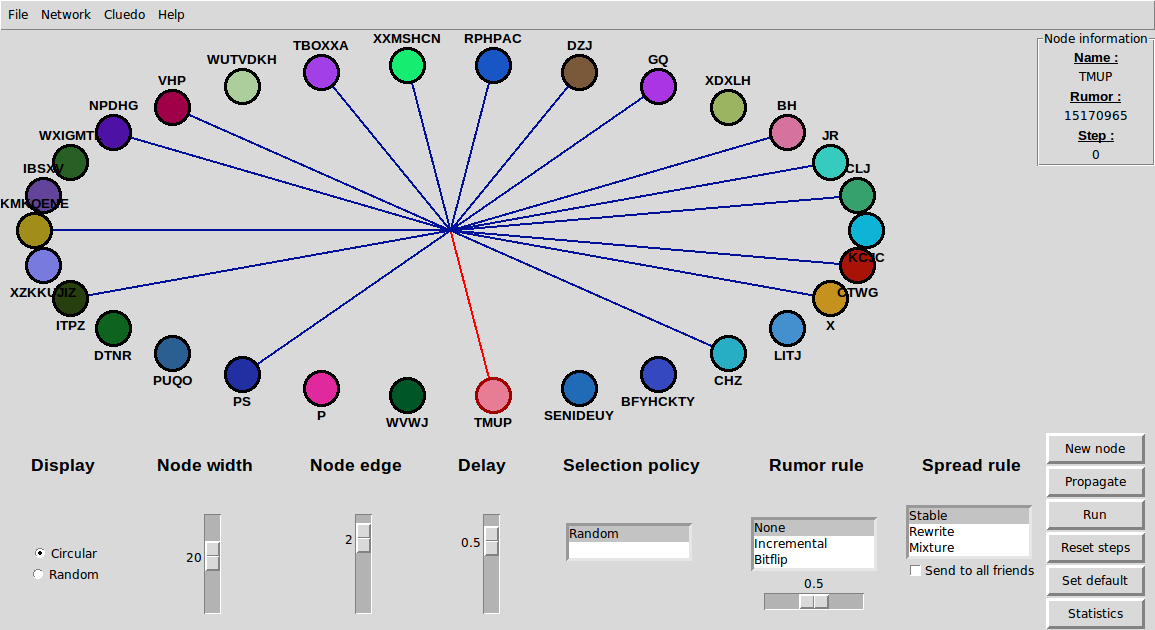
\includegraphics[width=17cm]{ReseauSimple.png}
\subsubsection{Exemple de création de lien d'amitié}
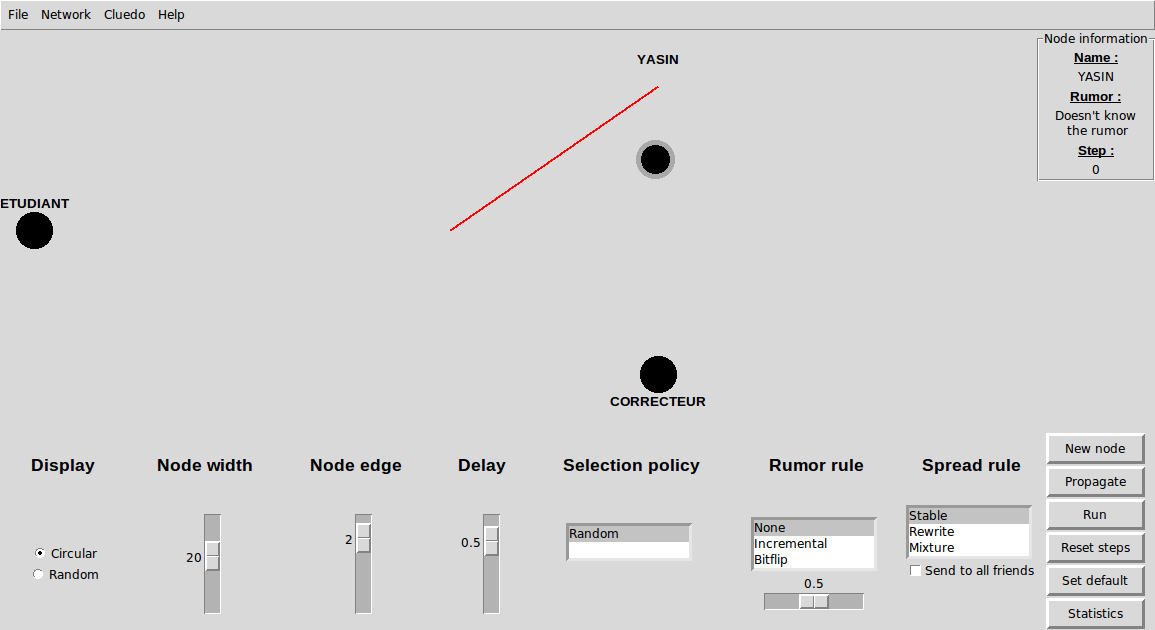
\includegraphics[width=17cm]{Relation.png}
\subsubsection{Statistiques d'un réseau}
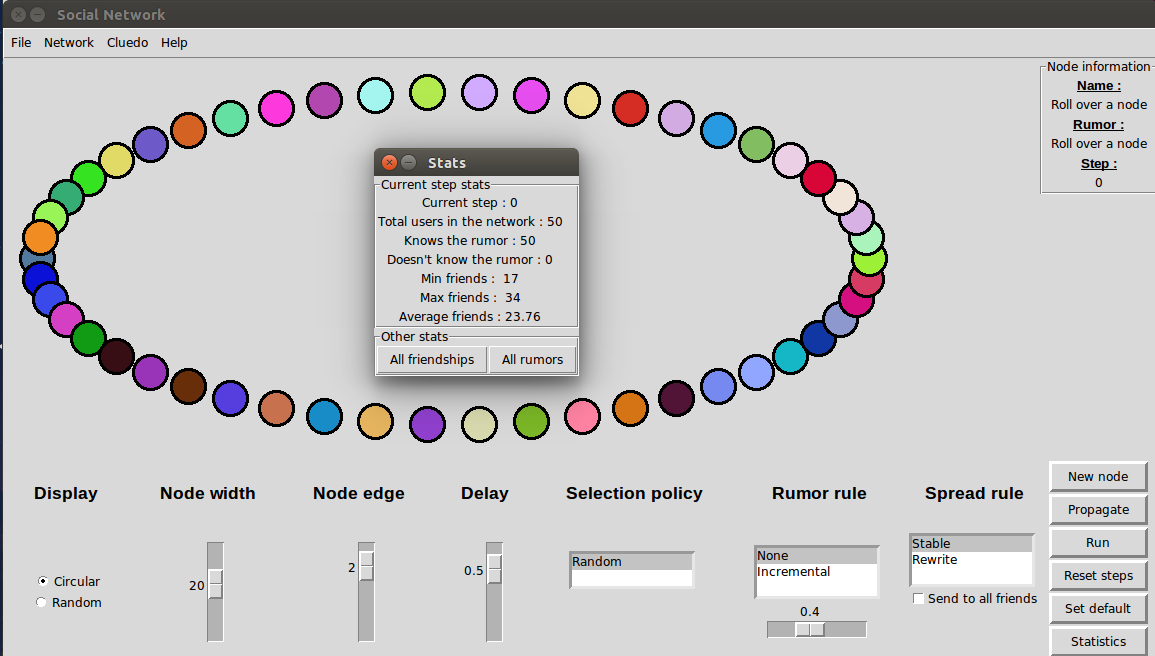
\includegraphics[width=17cm]{Stats.png}
\subsubsection{Modification possible du Cluedo}
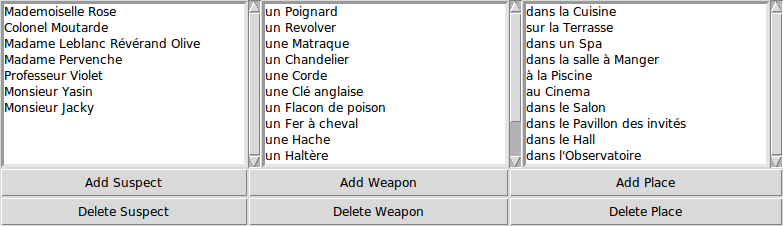
\includegraphics[width=17cm]{ModifyCluedo.png}

\section {Conclusion}
{Nous sommes capables maintenant de créer un réseau et d'y rependre une rumeur avec des options définis.
Ce rapport a résumé la manière dont j'ai réalisé les 4 grandes parties du projet, les choix que j'ai fait ainsi que les raisons.
L'affichage et l'exécution est soit sur terminal soit via interface graphique. Le travail a été codé comme suit les règles 
de l'énoncé. Les structures ont été respectées même si certains auraient pu être plus efficaces.
Nous, étudiant en BA1 sciences informatiques à l'ULB, nous n'avons jamais écrit de code aussi long. Ce projet nous a permis 
de gerer un code de plus de 1000 lignes. Il fallait également gérer le temps pour faire parvenir les parties dans les temps.
En parallèle du cours d'algorithmique et de programmation, nous avons appris les classes. Et depuis cette base, 
il nous a été demandé de nous documenter par nous même pour apprendre l'utilisation de Tkinter. Aucun cours ne nous a été donné.
Pour m'aider à réaliser tout ce projet, le bouquin de Gerard Swinnen : Apprendre à programmer avec python 3 était là pour combler mes manques.
Comme conclusion finale, nous avons appris que le bouche à oreille est une pratique risqué.}
\end{document}